\documentclass[twoside]{book}

% Packages required by doxygen
\usepackage{fixltx2e}
\usepackage{calc}
\usepackage{doxygen}
\usepackage[export]{adjustbox} % also loads graphicx
\usepackage{graphicx}
\usepackage[utf8]{inputenc}
\usepackage{makeidx}
\usepackage{multicol}
\usepackage{multirow}
\PassOptionsToPackage{warn}{textcomp}
\usepackage{textcomp}
\usepackage[nointegrals]{wasysym}
\usepackage[table]{xcolor}

% NLS support packages
\usepackage[french]{babel}

% Font selection
\usepackage[T1]{fontenc}
\usepackage[scaled=.90]{helvet}
\usepackage{courier}
\usepackage{amssymb}
\usepackage{sectsty}
\renewcommand{\familydefault}{\sfdefault}
\allsectionsfont{%
  \fontseries{bc}\selectfont%
  \color{darkgray}%
}
\renewcommand{\DoxyLabelFont}{%
  \fontseries{bc}\selectfont%
  \color{darkgray}%
}
\newcommand{\+}{\discretionary{\mbox{\scriptsize$\hookleftarrow$}}{}{}}

% Page & text layout
\usepackage{geometry}
\geometry{%
  a4paper,%
  top=2.5cm,%
  bottom=2.5cm,%
  left=2.5cm,%
  right=2.5cm%
}
\tolerance=750
\hfuzz=15pt
\hbadness=750
\setlength{\emergencystretch}{15pt}
\setlength{\parindent}{0cm}
\setlength{\parskip}{3ex plus 2ex minus 2ex}
\makeatletter
\renewcommand{\paragraph}{%
  \@startsection{paragraph}{4}{0ex}{-1.0ex}{1.0ex}{%
    \normalfont\normalsize\bfseries\SS@parafont%
  }%
}
\renewcommand{\subparagraph}{%
  \@startsection{subparagraph}{5}{0ex}{-1.0ex}{1.0ex}{%
    \normalfont\normalsize\bfseries\SS@subparafont%
  }%
}
\makeatother

% Headers & footers
\usepackage{fancyhdr}
\pagestyle{fancyplain}
\fancyhead[LE]{\fancyplain{}{\bfseries\thepage}}
\fancyhead[CE]{\fancyplain{}{}}
\fancyhead[RE]{\fancyplain{}{\bfseries\leftmark}}
\fancyhead[LO]{\fancyplain{}{\bfseries\rightmark}}
\fancyhead[CO]{\fancyplain{}{}}
\fancyhead[RO]{\fancyplain{}{\bfseries\thepage}}
\fancyfoot[LE]{\fancyplain{}{}}
\fancyfoot[CE]{\fancyplain{}{}}
\fancyfoot[RE]{\fancyplain{}{\bfseries\scriptsize Généré par Doxygen }}
\fancyfoot[LO]{\fancyplain{}{\bfseries\scriptsize Généré par Doxygen }}
\fancyfoot[CO]{\fancyplain{}{}}
\fancyfoot[RO]{\fancyplain{}{}}
\renewcommand{\footrulewidth}{0.4pt}
\renewcommand{\chaptermark}[1]{%
  \markboth{#1}{}%
}
\renewcommand{\sectionmark}[1]{%
  \markright{\thesection\ #1}%
}

% Indices & bibliography
\usepackage{natbib}
\usepackage[titles]{tocloft}
\setcounter{tocdepth}{3}
\setcounter{secnumdepth}{5}
\makeindex

% Hyperlinks (required, but should be loaded last)
\usepackage{ifpdf}
\ifpdf
  \usepackage[pdftex,pagebackref=true]{hyperref}
\else
  \usepackage[ps2pdf,pagebackref=true]{hyperref}
\fi
\hypersetup{%
  colorlinks=true,%
  linkcolor=blue,%
  citecolor=blue,%
  unicode%
}

% Custom commands
\newcommand{\clearemptydoublepage}{%
  \newpage{\pagestyle{empty}\cleardoublepage}%
}

\usepackage{caption}
\captionsetup{labelsep=space,justification=centering,font={bf},singlelinecheck=off,skip=4pt,position=top}

%===== C O N T E N T S =====

\begin{document}

% Titlepage & ToC
\hypersetup{pageanchor=false,
             bookmarksnumbered=true,
             pdfencoding=unicode
            }
\pagenumbering{roman}
\begin{titlepage}
\vspace*{7cm}
\begin{center}%
{\Large S\+H\+E\+LL Bourouis Heil }\\
\vspace*{1cm}
{\large Généré par Doxygen 1.8.11}\\
\end{center}
\end{titlepage}
\clearemptydoublepage
\tableofcontents
\clearemptydoublepage
\pagenumbering{arabic}
\hypersetup{pageanchor=true}

%--- Begin generated contents ---
\chapter{Index des structures de données}
\section{Structures de données}
Liste des structures de données avec une brève description \+:\begin{DoxyCompactList}
\item\contentsline{section}{\hyperlink{structELT}{E\+LT} }{\pageref{structELT}}{}
\item\contentsline{section}{\hyperlink{structLISTE}{L\+I\+S\+TE} }{\pageref{structLISTE}}{}
\item\contentsline{section}{\hyperlink{structNOEUD}{N\+O\+E\+UD} }{\pageref{structNOEUD}}{}
\end{DoxyCompactList}

\chapter{Index des fichiers}
\section{Liste des fichiers}
Liste de tous les fichiers documentés avec une brève description \+:\begin{DoxyCompactList}
\item\contentsline{section}{include/{\bfseries arbr.\+h} }{\pageref{arbr_8h}}{}
\item\contentsline{section}{include/{\bfseries builtin.\+h} }{\pageref{builtin_8h}}{}
\item\contentsline{section}{include/{\bfseries liste\+\_\+chaine.\+h} }{\pageref{liste__chaine_8h}}{}
\item\contentsline{section}{include/{\bfseries String\+Goodies.\+h} }{\pageref{StringGoodies_8h}}{}
\item\contentsline{section}{src/\hyperlink{arbr_8c}{arbr.\+c} \\*Implementation des arbres binaires }{\pageref{arbr_8c}}{}
\item\contentsline{section}{src/\hyperlink{builtin_8c}{builtin.\+c} \\*Fichier permettant de lancer un Mini\+Shell }{\pageref{builtin_8c}}{}
\item\contentsline{section}{src/\hyperlink{skeleton_8c}{skeleton.\+c} \\*Fichier permettant de lancer un Mini\+Shell }{\pageref{skeleton_8c}}{}
\item\contentsline{section}{src/\hyperlink{StringGoodies_8c}{String\+Goodies.\+c} \\*Fichier utilitaire créer pour faciliter le traitement des chaînes de caractères }{\pageref{StringGoodies_8c}}{}
\end{DoxyCompactList}

\chapter{Documentation des structures de données}
\hypertarget{structELT}{}\section{Référence de la structure E\+LT}
\label{structELT}\index{E\+LT@{E\+LT}}


Graphe de collaboration de E\+LT\+:
\nopagebreak
\begin{figure}[H]
\begin{center}
\leavevmode
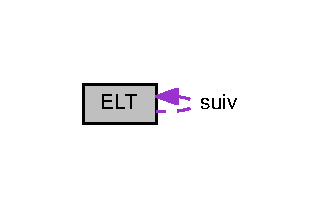
\includegraphics[width=155pt]{structELT__coll__graph}
\end{center}
\end{figure}
\subsection*{Champs de données}
\begin{DoxyCompactItemize}
\item 
char {\bfseries val}\hypertarget{structELT_a1fe6eedb2f252bbad8a996701512900e}{}\label{structELT_a1fe6eedb2f252bbad8a996701512900e}

\item 
struct \hyperlink{structELT}{E\+LT} $\ast$ {\bfseries suiv}\hypertarget{structELT_ae71c884a097920444cc50682340d4b31}{}\label{structELT_ae71c884a097920444cc50682340d4b31}

\end{DoxyCompactItemize}


La documentation de cette structure a été générée à partir du fichier suivant \+:\begin{DoxyCompactItemize}
\item 
include/liste\+\_\+chaine.\+h\end{DoxyCompactItemize}

\hypertarget{structLISTE}{}\section{Référence de la structure L\+I\+S\+TE}
\label{structLISTE}\index{L\+I\+S\+TE@{L\+I\+S\+TE}}


Graphe de collaboration de L\+I\+S\+TE\+:
\nopagebreak
\begin{figure}[H]
\begin{center}
\leavevmode
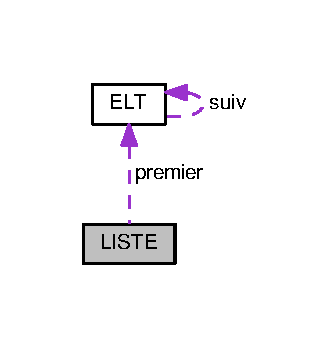
\includegraphics[width=160pt]{structLISTE__coll__graph}
\end{center}
\end{figure}
\subsection*{Champs de données}
\begin{DoxyCompactItemize}
\item 
\hyperlink{structELT}{elt\+\_\+liste} {\bfseries premier}\hypertarget{structLISTE_a6cd2848fc95de0497e8da669bd46ceb4}{}\label{structLISTE_a6cd2848fc95de0497e8da669bd46ceb4}

\end{DoxyCompactItemize}


La documentation de cette structure a été générée à partir du fichier suivant \+:\begin{DoxyCompactItemize}
\item 
include/liste\+\_\+chaine.\+h\end{DoxyCompactItemize}

\hypertarget{structNOEUD}{}\section{Référence de la structure N\+O\+E\+UD}
\label{structNOEUD}\index{N\+O\+E\+UD@{N\+O\+E\+UD}}


Graphe de collaboration de N\+O\+E\+UD\+:
\nopagebreak
\begin{figure}[H]
\begin{center}
\leavevmode
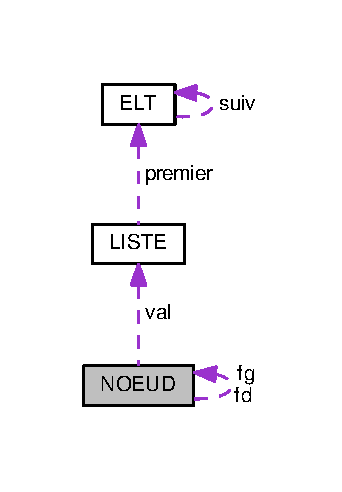
\includegraphics[width=164pt]{structNOEUD__coll__graph}
\end{center}
\end{figure}
\subsection*{Champs de données}
\begin{DoxyCompactItemize}
\item 
\hyperlink{structLISTE}{T} {\bfseries val}\hypertarget{structNOEUD_a028a6db155a103060682adbecd1d096b}{}\label{structNOEUD_a028a6db155a103060682adbecd1d096b}

\item 
struct \hyperlink{structNOEUD}{N\+O\+E\+UD} $\ast$ {\bfseries fg}\hypertarget{structNOEUD_a051a743170965d9dfe5fa55b6c883f9a}{}\label{structNOEUD_a051a743170965d9dfe5fa55b6c883f9a}

\item 
struct \hyperlink{structNOEUD}{N\+O\+E\+UD} $\ast$ {\bfseries fd}\hypertarget{structNOEUD_aa4c90a057bed56b598c16a5d9a12809e}{}\label{structNOEUD_aa4c90a057bed56b598c16a5d9a12809e}

\end{DoxyCompactItemize}


La documentation de cette structure a été générée à partir du fichier suivant \+:\begin{DoxyCompactItemize}
\item 
include/arbr.\+h\end{DoxyCompactItemize}

\chapter{Documentation des fichiers}
\hypertarget{arbr_8c}{}\section{Référence du fichier src/arbr.c}
\label{arbr_8c}\index{src/arbr.\+c@{src/arbr.\+c}}


Implementation des arbres binaires.  


{\ttfamily \#include $<$stdio.\+h$>$}\\*
{\ttfamily \#include $<$stdlib.\+h$>$}\\*
{\ttfamily \#include \char`\"{}arbr.\+h\char`\"{}}\\*
Graphe des dépendances par inclusion de arbr.\+c\+:
\nopagebreak
\begin{figure}[H]
\begin{center}
\leavevmode
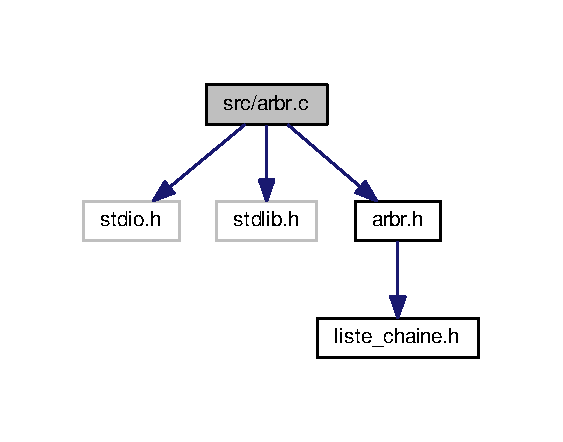
\includegraphics[width=270pt]{arbr_8c__incl}
\end{center}
\end{figure}
\subsection*{Fonctions}
\begin{DoxyCompactItemize}
\item 
\hyperlink{structNOEUD}{arbre} \hyperlink{arbr_8c_a6e9a2f685eb2b497e2515d99d64f1707}{nouv\+Arbre} ()
\item 
\hyperlink{structNOEUD}{arbre} \hyperlink{arbr_8c_a5b331779e8516a499cf3fd3f9482b639}{enracA} (\hyperlink{structLISTE}{T} racine, \hyperlink{structNOEUD}{arbre} fg, \hyperlink{structNOEUD}{arbre} fd)
\item 
\hyperlink{structNOEUD}{arbre} \hyperlink{arbr_8c_a94f09e4f4f13809eaa12e06f7a2f1c25}{creer\+FeuilleA} (\hyperlink{structLISTE}{T} val)
\item 
\hyperlink{structLISTE}{T} \hyperlink{arbr_8c_ab8442ac3359628e2ccec0ff0b0d66ad6}{racineA} (\hyperlink{structNOEUD}{arbre} a)
\item 
\hyperlink{structNOEUD}{arbre} \hyperlink{arbr_8c_a1a58318786f1702a130528f1858f3aab}{fgA} (\hyperlink{structNOEUD}{arbre} a)
\item 
\hyperlink{structNOEUD}{arbre} \hyperlink{arbr_8c_aa35dd5636be08efc9f91803028350ed6}{fdA} (\hyperlink{structNOEUD}{arbre} a)
\item 
int \hyperlink{arbr_8c_a2841559f65f98f60e637e89d333735e2}{est\+VideA} (\hyperlink{structNOEUD}{arbre} a)
\item 
void \hyperlink{arbr_8c_a59755441984d17f00cf42b373043902c}{parcours\+PrefixeA} (\hyperlink{structNOEUD}{arbre} a, void($\ast$affiche)(\hyperlink{structLISTE}{T}))
\end{DoxyCompactItemize}


\subsection{Description détaillée}
Implementation des arbres binaires. 

\begin{DoxyAuthor}{Auteur}
Alexis Heil, Sabrina Bourouis 
\end{DoxyAuthor}
\begin{DoxyVersion}{Version}
0.\+1 
\end{DoxyVersion}
\begin{DoxyDate}{Date}
09 fevrier 2017
\end{DoxyDate}
Implementation des arbres binaires 

\subsection{Documentation des fonctions}
\index{arbr.\+c@{arbr.\+c}!creer\+FeuilleA@{creer\+FeuilleA}}
\index{creer\+FeuilleA@{creer\+FeuilleA}!arbr.\+c@{arbr.\+c}}
\subsubsection[{\texorpdfstring{creer\+Feuille\+A(\+T val)}{creerFeuilleA(T val)}}]{\setlength{\rightskip}{0pt plus 5cm}{\bf arbre} creer\+FeuilleA (
\begin{DoxyParamCaption}
\item[{{\bf T}}]{val}
\end{DoxyParamCaption}
)}\hypertarget{arbr_8c_a94f09e4f4f13809eaa12e06f7a2f1c25}{}\label{arbr_8c_a94f09e4f4f13809eaa12e06f7a2f1c25}
Fonction permettant de creer une feuille \+: un arbre avec une branche droite et une branche gauche egale a null


\begin{DoxyParams}{Paramètres}
{\em T} & val valeur de la feuille a creer \\
\hline
\end{DoxyParams}
\begin{DoxyReturn}{Renvoie}
arbre renvoie un pointeur sur la feuille creee 
\end{DoxyReturn}
\index{arbr.\+c@{arbr.\+c}!enracA@{enracA}}
\index{enracA@{enracA}!arbr.\+c@{arbr.\+c}}
\subsubsection[{\texorpdfstring{enrac\+A(\+T racine, arbre fg, arbre fd)}{enracA(T racine, arbre fg, arbre fd)}}]{\setlength{\rightskip}{0pt plus 5cm}{\bf arbre} enracA (
\begin{DoxyParamCaption}
\item[{{\bf T}}]{racine, }
\item[{{\bf arbre}}]{fg, }
\item[{{\bf arbre}}]{fd}
\end{DoxyParamCaption}
)}\hypertarget{arbr_8c_a5b331779e8516a499cf3fd3f9482b639}{}\label{arbr_8c_a5b331779e8516a499cf3fd3f9482b639}
Fonction permettant de creer un nouvelle arbre en ajoutant une valeur a la racine et en lui specifiant les differentes branches


\begin{DoxyParams}{Paramètres}
{\em T} & racine valeur du noeud racine \\
\hline
{\em arbre} & fg feuille gauche de l\textquotesingle{}arbre \\
\hline
{\em arbre} & fd feuille droite de l\textquotesingle{}arbre \\
\hline
\end{DoxyParams}
\begin{DoxyReturn}{Renvoie}
arbre renvoie un pointeur sur le noeud racine 
\end{DoxyReturn}
\index{arbr.\+c@{arbr.\+c}!est\+VideA@{est\+VideA}}
\index{est\+VideA@{est\+VideA}!arbr.\+c@{arbr.\+c}}
\subsubsection[{\texorpdfstring{est\+Vide\+A(arbre a)}{estVideA(arbre a)}}]{\setlength{\rightskip}{0pt plus 5cm}int est\+VideA (
\begin{DoxyParamCaption}
\item[{{\bf arbre}}]{a}
\end{DoxyParamCaption}
)}\hypertarget{arbr_8c_a2841559f65f98f60e637e89d333735e2}{}\label{arbr_8c_a2841559f65f98f60e637e89d333735e2}
Fonction permettant de savoir si un arbre est vide ou non


\begin{DoxyParams}{Paramètres}
{\em arbre} & a pointeur sur l\textquotesingle{}arbre dont on souhaite verifier s\textquotesingle{}il est vide ou pas \\
\hline
\end{DoxyParams}
\begin{DoxyReturn}{Renvoie}
int renvoie 1 si a est null, 0 sinon 
\end{DoxyReturn}
\index{arbr.\+c@{arbr.\+c}!fdA@{fdA}}
\index{fdA@{fdA}!arbr.\+c@{arbr.\+c}}
\subsubsection[{\texorpdfstring{fd\+A(arbre a)}{fdA(arbre a)}}]{\setlength{\rightskip}{0pt plus 5cm}{\bf arbre} fdA (
\begin{DoxyParamCaption}
\item[{{\bf arbre}}]{a}
\end{DoxyParamCaption}
)}\hypertarget{arbr_8c_aa35dd5636be08efc9f91803028350ed6}{}\label{arbr_8c_aa35dd5636be08efc9f91803028350ed6}
Fonction permettant de reccuperer la valeur de la feuille droite d\textquotesingle{}un arbre


\begin{DoxyParams}{Paramètres}
{\em arbre} & a pointeur sur l\textquotesingle{}arbre dont on souhaite recuperer la feuille droite \\
\hline
\end{DoxyParams}
\begin{DoxyReturn}{Renvoie}
arbre renvoie la feuille droite de l\textquotesingle{}arbre passe en parametre 
\end{DoxyReturn}
\index{arbr.\+c@{arbr.\+c}!fgA@{fgA}}
\index{fgA@{fgA}!arbr.\+c@{arbr.\+c}}
\subsubsection[{\texorpdfstring{fg\+A(arbre a)}{fgA(arbre a)}}]{\setlength{\rightskip}{0pt plus 5cm}{\bf arbre} fgA (
\begin{DoxyParamCaption}
\item[{{\bf arbre}}]{a}
\end{DoxyParamCaption}
)}\hypertarget{arbr_8c_a1a58318786f1702a130528f1858f3aab}{}\label{arbr_8c_a1a58318786f1702a130528f1858f3aab}
Fonction permettant de reccuperer la valeur de la feuille gauche d\textquotesingle{}un arbre


\begin{DoxyParams}{Paramètres}
{\em arbre} & a pointeur sur l\textquotesingle{}arbre dont on souhaite recuperer la feuille gauche \\
\hline
\end{DoxyParams}
\begin{DoxyReturn}{Renvoie}
arbre renvoie la feuille gauche de l\textquotesingle{}arbre passe en parametre 
\end{DoxyReturn}
\index{arbr.\+c@{arbr.\+c}!nouv\+Arbre@{nouv\+Arbre}}
\index{nouv\+Arbre@{nouv\+Arbre}!arbr.\+c@{arbr.\+c}}
\subsubsection[{\texorpdfstring{nouv\+Arbre()}{nouvArbre()}}]{\setlength{\rightskip}{0pt plus 5cm}{\bf arbre} nouv\+Arbre (
\begin{DoxyParamCaption}
{}
\end{DoxyParamCaption}
)}\hypertarget{arbr_8c_a6e9a2f685eb2b497e2515d99d64f1707}{}\label{arbr_8c_a6e9a2f685eb2b497e2515d99d64f1707}
Fonction permettant de creer un arbre vide

\begin{DoxyReturn}{Renvoie}
arbre renvoie N\+U\+LL 
\end{DoxyReturn}
\index{arbr.\+c@{arbr.\+c}!parcours\+PrefixeA@{parcours\+PrefixeA}}
\index{parcours\+PrefixeA@{parcours\+PrefixeA}!arbr.\+c@{arbr.\+c}}
\subsubsection[{\texorpdfstring{parcours\+Prefixe\+A(arbre a, void($\ast$affiche)(\+T))}{parcoursPrefixeA(arbre a, void(*affiche)(T))}}]{\setlength{\rightskip}{0pt plus 5cm}void parcours\+PrefixeA (
\begin{DoxyParamCaption}
\item[{{\bf arbre}}]{a, }
\item[{void($\ast$)({\bf T})}]{affiche}
\end{DoxyParamCaption}
)}\hypertarget{arbr_8c_a59755441984d17f00cf42b373043902c}{}\label{arbr_8c_a59755441984d17f00cf42b373043902c}
Fonction permettant d\textquotesingle{}appliquer une fonction sur chacun des noeud en parcourant l\textquotesingle{}arbre de façon prefixe


\begin{DoxyParams}{Paramètres}
{\em arbre} & a pointeur sur l\textquotesingle{}arbre a parcourir \\
\hline
{\em void} & $\ast$affiche pointeur sur une fonction qui prend un parametre T \\
\hline
\end{DoxyParams}
\index{arbr.\+c@{arbr.\+c}!racineA@{racineA}}
\index{racineA@{racineA}!arbr.\+c@{arbr.\+c}}
\subsubsection[{\texorpdfstring{racine\+A(arbre a)}{racineA(arbre a)}}]{\setlength{\rightskip}{0pt plus 5cm}{\bf T} racineA (
\begin{DoxyParamCaption}
\item[{{\bf arbre}}]{a}
\end{DoxyParamCaption}
)}\hypertarget{arbr_8c_ab8442ac3359628e2ccec0ff0b0d66ad6}{}\label{arbr_8c_ab8442ac3359628e2ccec0ff0b0d66ad6}
Fonction permettant de reccuperer la valeur du noeud racine


\begin{DoxyParams}{Paramètres}
{\em arbre} & a pointeur sur la racine de l\textquotesingle{}arbre \\
\hline
\end{DoxyParams}
\begin{DoxyReturn}{Renvoie}
T renvoie la valeur du noeud racine 
\end{DoxyReturn}

\hypertarget{builtin_8c}{}\section{Référence du fichier src/builtin.c}
\label{builtin_8c}\index{src/builtin.\+c@{src/builtin.\+c}}


Fichier permettant de lancer un Mini\+Shell.  


{\ttfamily \#include $<$stdio.\+h$>$}\\*
{\ttfamily \#include $<$stdlib.\+h$>$}\\*
{\ttfamily \#include $<$sys/stat.\+h$>$}\\*
{\ttfamily \#include $<$fcntl.\+h$>$}\\*
{\ttfamily \#include $<$string.\+h$>$}\\*
{\ttfamily \#include $<$unistd.\+h$>$}\\*
{\ttfamily \#include $<$String\+Goodies.\+h$>$}\\*
{\ttfamily \#include \char`\"{}builtin.\+h\char`\"{}}\\*
Graphe des dépendances par inclusion de builtin.\+c\+:
\nopagebreak
\begin{figure}[H]
\begin{center}
\leavevmode
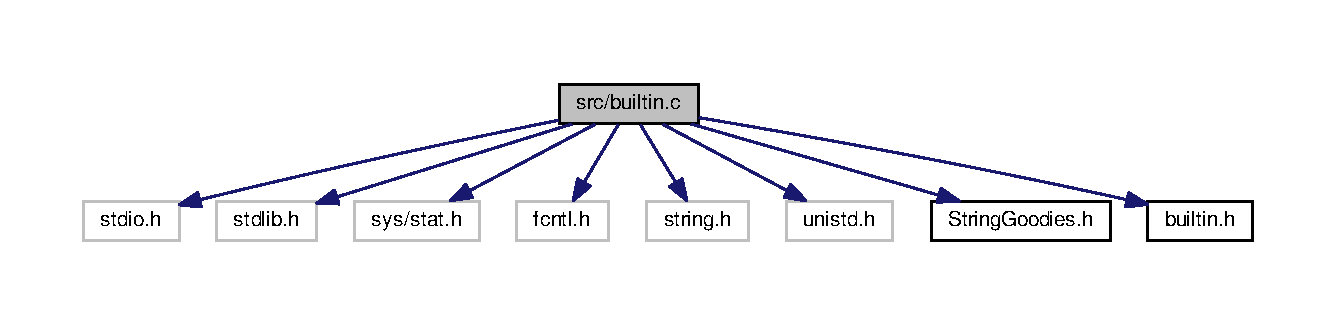
\includegraphics[width=350pt]{builtin_8c__incl}
\end{center}
\end{figure}
\subsection*{Fonctions}
\begin{DoxyCompactItemize}
\item 
int \hyperlink{builtin_8c_aee04a4727da3087227ee83278b12c351}{lsh\+\_\+num\+\_\+builtins} ()
\begin{DoxyCompactList}\small\item\em fonction qui retourne le nombre d\textquotesingle{}element dans le tableau builtin\+\_\+str \end{DoxyCompactList}\item 
int \hyperlink{builtin_8c_ac358e0686c4942b1ccf21b44ee4e7abc}{lsh\+\_\+cd} (char $\ast$$\ast$args)
\begin{DoxyCompactList}\small\item\em fonction qui correspond a l\textquotesingle{}implementation de la fonction cd \end{DoxyCompactList}\item 
int \hyperlink{builtin_8c_ad4b8db0d9ff9cc2f8969d06667efef6b}{lsh\+\_\+help} (char $\ast$$\ast$args)
\begin{DoxyCompactList}\small\item\em fonction qui correspond a l\textquotesingle{}implementation de la fonction help \end{DoxyCompactList}\item 
int \hyperlink{builtin_8c_a922a56166c20f5a20209c29efbfaf8fd}{lsh\+\_\+exit} (char $\ast$$\ast$args)
\begin{DoxyCompactList}\small\item\em fonction qui correspond a l\textquotesingle{}implementation de la fonction exit \end{DoxyCompactList}\item 
int \hyperlink{builtin_8c_a1de142ca492ac2801531c75edc404cd6}{lsh\+\_\+pwd} (char $\ast$$\ast$args)
\begin{DoxyCompactList}\small\item\em fonction qui correspond a l\textquotesingle{}implementation de la fonction pwd \end{DoxyCompactList}\item 
int \hyperlink{builtin_8c_ac7048ea4c2e6f715237a4f2db844b03d}{lsh\+\_\+echo} (char $\ast$$\ast$args)
\begin{DoxyCompactList}\small\item\em fonction qui correspond a l\textquotesingle{}implementation de la fonction echo \end{DoxyCompactList}\item 
int \hyperlink{builtin_8c_aa2d59711ff0ae6aa4a3cc7b20894ef71}{lsh\+\_\+history} (char $\ast$$\ast$args)
\begin{DoxyCompactList}\small\item\em fonction qui correspond a l\textquotesingle{}implementation de la fonction history \end{DoxyCompactList}\item 
int \hyperlink{builtin_8c_aca0aefccee25b76d20a1fb12b7b1fb2a}{exec\+Builtin} (char $\ast$arg)
\begin{DoxyCompactList}\small\item\em fonction qui permet de selectionner la bonne commande builtin a executer \end{DoxyCompactList}\end{DoxyCompactItemize}
\subsection*{Variables}
\begin{DoxyCompactItemize}
\item 
char $\ast$ \hyperlink{builtin_8c_a37a367439f3da1f701aea106d2ae15c2}{builtin\+\_\+str} \mbox{[}$\,$\mbox{]}
\begin{DoxyCompactList}\small\item\em Tableau de char$\ast$ qui contient les differentes commandes qui ont ete implementees directement. \end{DoxyCompactList}\item 
int($\ast$ \hyperlink{builtin_8c_aa69e593df077eba1b3ebca24fc4afe05}{builtin\+\_\+func} \mbox{[}$\,$\mbox{]})(char $\ast$$\ast$)
\begin{DoxyCompactList}\small\item\em Tableau de pointeur de fonctions qui retourne un int et prenne un char $\ast$$\ast$ en parametre. Chacune de ces fonctions correspond a une des commandes implementees directement. \end{DoxyCompactList}\end{DoxyCompactItemize}


\subsection{Description détaillée}
Fichier permettant de lancer un Mini\+Shell. 

\begin{DoxyAuthor}{Auteur}
Alexis Heil, Sabrina Bourouis 
\end{DoxyAuthor}
\begin{DoxyVersion}{Version}
0.\+1 
\end{DoxyVersion}
\begin{DoxyDate}{Date}
09 fevrier 2017
\end{DoxyDate}
Mini Shell de Sabrina Bourouis et Alexis Heil 

\subsection{Documentation des fonctions}
\index{builtin.\+c@{builtin.\+c}!exec\+Builtin@{exec\+Builtin}}
\index{exec\+Builtin@{exec\+Builtin}!builtin.\+c@{builtin.\+c}}
\subsubsection[{\texorpdfstring{exec\+Builtin(char $\ast$arg)}{execBuiltin(char *arg)}}]{\setlength{\rightskip}{0pt plus 5cm}int exec\+Builtin (
\begin{DoxyParamCaption}
\item[{char $\ast$}]{arg}
\end{DoxyParamCaption}
)}\hypertarget{builtin_8c_aca0aefccee25b76d20a1fb12b7b1fb2a}{}\label{builtin_8c_aca0aefccee25b76d20a1fb12b7b1fb2a}


fonction qui permet de selectionner la bonne commande builtin a executer 


\begin{DoxyParams}{Paramètres}
{\em char} & $\ast$ args argument de la commande a executer le premier element du tableau est history \mbox{[}Pas utilise juste pour correspondre a la definition du tableau de fonction\mbox{]} \\
\hline
\end{DoxyParams}
\begin{DoxyReturn}{Renvoie}
int code retour de la fonction 1 si la fonction se termine bien et 0 sinon 
\end{DoxyReturn}
\index{builtin.\+c@{builtin.\+c}!lsh\+\_\+cd@{lsh\+\_\+cd}}
\index{lsh\+\_\+cd@{lsh\+\_\+cd}!builtin.\+c@{builtin.\+c}}
\subsubsection[{\texorpdfstring{lsh\+\_\+cd(char $\ast$$\ast$args)}{lsh_cd(char **args)}}]{\setlength{\rightskip}{0pt plus 5cm}int lsh\+\_\+cd (
\begin{DoxyParamCaption}
\item[{char $\ast$$\ast$}]{args}
\end{DoxyParamCaption}
)}\hypertarget{builtin_8c_ac358e0686c4942b1ccf21b44ee4e7abc}{}\label{builtin_8c_ac358e0686c4942b1ccf21b44ee4e7abc}


fonction qui correspond a l\textquotesingle{}implementation de la fonction cd 


\begin{DoxyParams}{Paramètres}
{\em char} & $\ast$$\ast$ args argument de la commande a executer le premier element du tableau est cd \\
\hline
\end{DoxyParams}
\begin{DoxyReturn}{Renvoie}
int code retour de la fonction 1 si la fonction se termine bien et 0 sinon 
\end{DoxyReturn}
\index{builtin.\+c@{builtin.\+c}!lsh\+\_\+echo@{lsh\+\_\+echo}}
\index{lsh\+\_\+echo@{lsh\+\_\+echo}!builtin.\+c@{builtin.\+c}}
\subsubsection[{\texorpdfstring{lsh\+\_\+echo(char $\ast$$\ast$args)}{lsh_echo(char **args)}}]{\setlength{\rightskip}{0pt plus 5cm}int lsh\+\_\+echo (
\begin{DoxyParamCaption}
\item[{char $\ast$$\ast$}]{args}
\end{DoxyParamCaption}
)}\hypertarget{builtin_8c_ac7048ea4c2e6f715237a4f2db844b03d}{}\label{builtin_8c_ac7048ea4c2e6f715237a4f2db844b03d}


fonction qui correspond a l\textquotesingle{}implementation de la fonction echo 


\begin{DoxyParams}{Paramètres}
{\em char} & $\ast$$\ast$ args argument de la commande a executer le premier element du tableau est echo \mbox{[}Pas utilise juste pour correspondre a la definition du tableau de fonction\mbox{]} \\
\hline
\end{DoxyParams}
\begin{DoxyReturn}{Renvoie}
int code retour de la fonction \+: 1 
\end{DoxyReturn}
\index{builtin.\+c@{builtin.\+c}!lsh\+\_\+exit@{lsh\+\_\+exit}}
\index{lsh\+\_\+exit@{lsh\+\_\+exit}!builtin.\+c@{builtin.\+c}}
\subsubsection[{\texorpdfstring{lsh\+\_\+exit(char $\ast$$\ast$args)}{lsh_exit(char **args)}}]{\setlength{\rightskip}{0pt plus 5cm}int lsh\+\_\+exit (
\begin{DoxyParamCaption}
\item[{char $\ast$$\ast$}]{args}
\end{DoxyParamCaption}
)}\hypertarget{builtin_8c_a922a56166c20f5a20209c29efbfaf8fd}{}\label{builtin_8c_a922a56166c20f5a20209c29efbfaf8fd}


fonction qui correspond a l\textquotesingle{}implementation de la fonction exit 


\begin{DoxyParams}{Paramètres}
{\em char} & $\ast$$\ast$ args argument de la commande a executer le premier element du tableau est exit \mbox{[}Pas utilise juste pour correspondre a la definition du tableau de fonction\mbox{]} \\
\hline
\end{DoxyParams}
\begin{DoxyReturn}{Renvoie}
int code retour de la fonction \+: 0 
\end{DoxyReturn}
\index{builtin.\+c@{builtin.\+c}!lsh\+\_\+help@{lsh\+\_\+help}}
\index{lsh\+\_\+help@{lsh\+\_\+help}!builtin.\+c@{builtin.\+c}}
\subsubsection[{\texorpdfstring{lsh\+\_\+help(char $\ast$$\ast$args)}{lsh_help(char **args)}}]{\setlength{\rightskip}{0pt plus 5cm}int lsh\+\_\+help (
\begin{DoxyParamCaption}
\item[{char $\ast$$\ast$}]{args}
\end{DoxyParamCaption}
)}\hypertarget{builtin_8c_ad4b8db0d9ff9cc2f8969d06667efef6b}{}\label{builtin_8c_ad4b8db0d9ff9cc2f8969d06667efef6b}


fonction qui correspond a l\textquotesingle{}implementation de la fonction help 


\begin{DoxyParams}{Paramètres}
{\em char} & $\ast$$\ast$ args argument de la commande a executer le premier element du tableau est help \\
\hline
\end{DoxyParams}
\begin{DoxyReturn}{Renvoie}
int code retour de la fonction \+: 1 (elle effectue juste un affichage) 
\end{DoxyReturn}
\index{builtin.\+c@{builtin.\+c}!lsh\+\_\+history@{lsh\+\_\+history}}
\index{lsh\+\_\+history@{lsh\+\_\+history}!builtin.\+c@{builtin.\+c}}
\subsubsection[{\texorpdfstring{lsh\+\_\+history(char $\ast$$\ast$args)}{lsh_history(char **args)}}]{\setlength{\rightskip}{0pt plus 5cm}int lsh\+\_\+history (
\begin{DoxyParamCaption}
\item[{char $\ast$$\ast$}]{args}
\end{DoxyParamCaption}
)}\hypertarget{builtin_8c_aa2d59711ff0ae6aa4a3cc7b20894ef71}{}\label{builtin_8c_aa2d59711ff0ae6aa4a3cc7b20894ef71}


fonction qui correspond a l\textquotesingle{}implementation de la fonction history 


\begin{DoxyParams}{Paramètres}
{\em char} & $\ast$$\ast$ args argument de la commande a executer le premier element du tableau est history \mbox{[}Pas utilise juste pour correspondre a la definition du tableau de fonction\mbox{]} \\
\hline
\end{DoxyParams}
\begin{DoxyReturn}{Renvoie}
int code retour de la fonction 1 si la fonction se termine bien et 0 sinon 
\end{DoxyReturn}
\index{builtin.\+c@{builtin.\+c}!lsh\+\_\+num\+\_\+builtins@{lsh\+\_\+num\+\_\+builtins}}
\index{lsh\+\_\+num\+\_\+builtins@{lsh\+\_\+num\+\_\+builtins}!builtin.\+c@{builtin.\+c}}
\subsubsection[{\texorpdfstring{lsh\+\_\+num\+\_\+builtins()}{lsh_num_builtins()}}]{\setlength{\rightskip}{0pt plus 5cm}int lsh\+\_\+num\+\_\+builtins (
\begin{DoxyParamCaption}
{}
\end{DoxyParamCaption}
)}\hypertarget{builtin_8c_aee04a4727da3087227ee83278b12c351}{}\label{builtin_8c_aee04a4727da3087227ee83278b12c351}


fonction qui retourne le nombre d\textquotesingle{}element dans le tableau builtin\+\_\+str 

\begin{DoxyReturn}{Renvoie}
int taille du tableau builtin\+\_\+str 
\end{DoxyReturn}
\index{builtin.\+c@{builtin.\+c}!lsh\+\_\+pwd@{lsh\+\_\+pwd}}
\index{lsh\+\_\+pwd@{lsh\+\_\+pwd}!builtin.\+c@{builtin.\+c}}
\subsubsection[{\texorpdfstring{lsh\+\_\+pwd(char $\ast$$\ast$args)}{lsh_pwd(char **args)}}]{\setlength{\rightskip}{0pt plus 5cm}int lsh\+\_\+pwd (
\begin{DoxyParamCaption}
\item[{char $\ast$$\ast$}]{args}
\end{DoxyParamCaption}
)}\hypertarget{builtin_8c_a1de142ca492ac2801531c75edc404cd6}{}\label{builtin_8c_a1de142ca492ac2801531c75edc404cd6}


fonction qui correspond a l\textquotesingle{}implementation de la fonction pwd 


\begin{DoxyParams}{Paramètres}
{\em char} & $\ast$$\ast$ args argument de la commande a executer le premier element du tableau est pwd \mbox{[}Pas utilise juste pour correspondre a la definition du tableau de fonction\mbox{]} \\
\hline
\end{DoxyParams}
\begin{DoxyReturn}{Renvoie}
int code retour de la fonction \+: 1 
\end{DoxyReturn}


\subsection{Documentation des variables}
\index{builtin.\+c@{builtin.\+c}!builtin\+\_\+func@{builtin\+\_\+func}}
\index{builtin\+\_\+func@{builtin\+\_\+func}!builtin.\+c@{builtin.\+c}}
\subsubsection[{\texorpdfstring{builtin\+\_\+func}{builtin_func}}]{\setlength{\rightskip}{0pt plus 5cm}int($\ast$ builtin\+\_\+func\mbox{[}$\,$\mbox{]})(char $\ast$$\ast$)}\hypertarget{builtin_8c_aa69e593df077eba1b3ebca24fc4afe05}{}\label{builtin_8c_aa69e593df077eba1b3ebca24fc4afe05}
{\bfseries Valeur initiale \+:}
\begin{DoxyCode}
= \{
  &\hyperlink{builtin_8c_ac358e0686c4942b1ccf21b44ee4e7abc}{lsh\_cd},
  &\hyperlink{builtin_8c_ad4b8db0d9ff9cc2f8969d06667efef6b}{lsh\_help},
  &\hyperlink{builtin_8c_a922a56166c20f5a20209c29efbfaf8fd}{lsh\_exit},
  &\hyperlink{builtin_8c_a1de142ca492ac2801531c75edc404cd6}{lsh\_pwd},
  &\hyperlink{builtin_8c_ac7048ea4c2e6f715237a4f2db844b03d}{lsh\_echo},
  &\hyperlink{builtin_8c_aa2d59711ff0ae6aa4a3cc7b20894ef71}{lsh\_history}
\}
\end{DoxyCode}


Tableau de pointeur de fonctions qui retourne un int et prenne un char $\ast$$\ast$ en parametre. Chacune de ces fonctions correspond a une des commandes implementees directement. 

\index{builtin.\+c@{builtin.\+c}!builtin\+\_\+str@{builtin\+\_\+str}}
\index{builtin\+\_\+str@{builtin\+\_\+str}!builtin.\+c@{builtin.\+c}}
\subsubsection[{\texorpdfstring{builtin\+\_\+str}{builtin_str}}]{\setlength{\rightskip}{0pt plus 5cm}char$\ast$ builtin\+\_\+str\mbox{[}$\,$\mbox{]}}\hypertarget{builtin_8c_a37a367439f3da1f701aea106d2ae15c2}{}\label{builtin_8c_a37a367439f3da1f701aea106d2ae15c2}
{\bfseries Valeur initiale \+:}
\begin{DoxyCode}
= \{
  \textcolor{stringliteral}{"cd"},
  \textcolor{stringliteral}{"help"},
  \textcolor{stringliteral}{"exit"},
  \textcolor{stringliteral}{"pwd"}, 
  \textcolor{stringliteral}{"echo"},
  \textcolor{stringliteral}{"history"}
\}
\end{DoxyCode}


Tableau de char$\ast$ qui contient les differentes commandes qui ont ete implementees directement. 


\hypertarget{skeleton_8c}{}\section{Référence du fichier src/skeleton.c}
\label{skeleton_8c}\index{src/skeleton.\+c@{src/skeleton.\+c}}


Fichier permettant de lancer un Mini\+Shell.  


{\ttfamily \#include $<$stdio.\+h$>$}\\*
{\ttfamily \#include $<$stdlib.\+h$>$}\\*
{\ttfamily \#include $<$string.\+h$>$}\\*
{\ttfamily \#include $<$errno.\+h$>$}\\*
{\ttfamily \#include $<$sys/types.\+h$>$}\\*
{\ttfamily \#include $<$sys/stat.\+h$>$}\\*
{\ttfamily \#include $<$getopt.\+h$>$}\\*
{\ttfamily \#include $<$fcntl.\+h$>$}\\*
{\ttfamily \#include $<$unistd.\+h$>$}\\*
{\ttfamily \#include $<$sys/wait.\+h$>$}\\*
{\ttfamily \#include $<$time.\+h$>$}\\*
{\ttfamily \#include $<$liste\+\_\+chaine.\+h$>$}\\*
{\ttfamily \#include $<$arbr.\+h$>$}\\*
{\ttfamily \#include $<$String\+Goodies.\+h$>$}\\*
{\ttfamily \#include $<$builtin.\+h$>$}\\*
{\ttfamily \#include $<$assert.\+h$>$}\\*
Graphe des dépendances par inclusion de skeleton.\+c\+:
\nopagebreak
\begin{figure}[H]
\begin{center}
\leavevmode
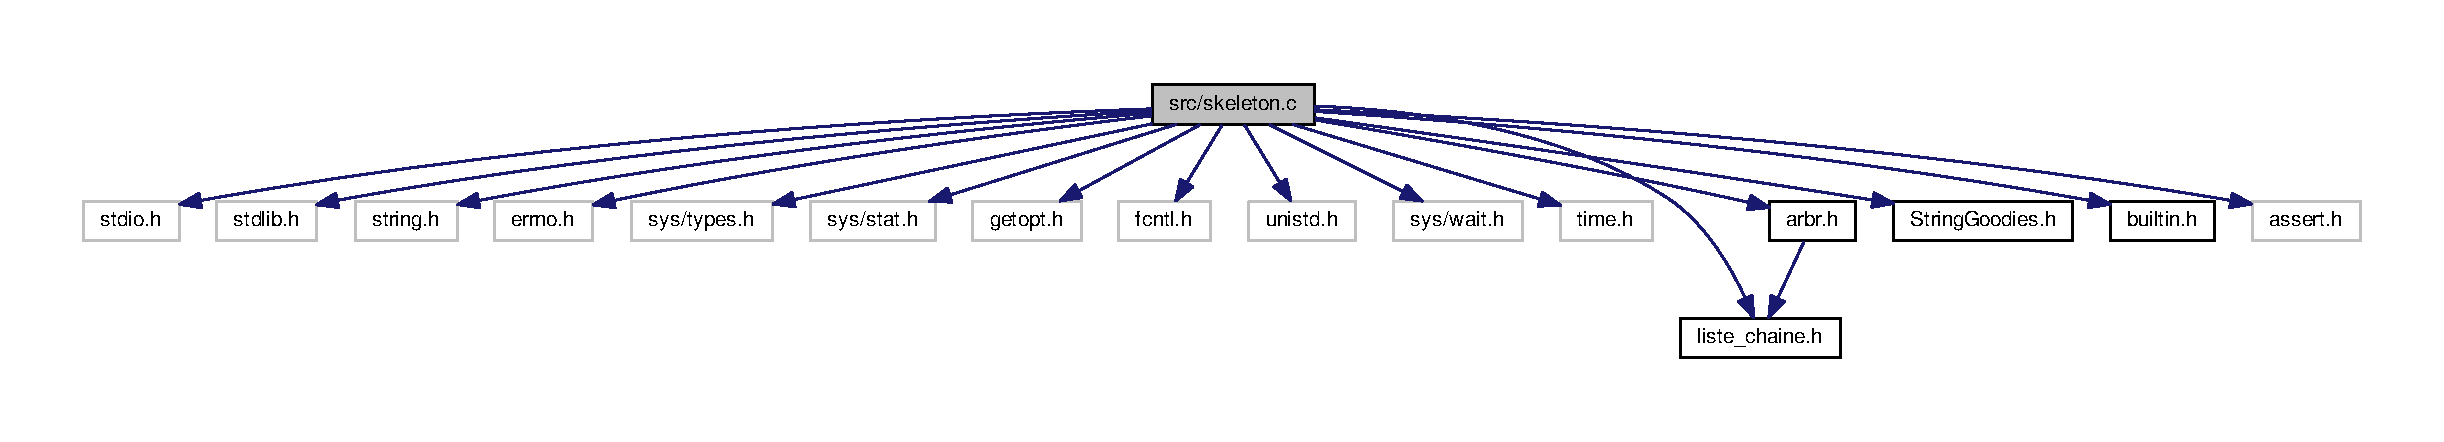
\includegraphics[width=350pt]{skeleton_8c__incl}
\end{center}
\end{figure}
\subsection*{Macros}
\begin{DoxyCompactItemize}
\item 
\#define {\bfseries C\+O\+P\+I\+E\+\_\+\+F\+I\+L\+E\+N\+A\+ME}~\char`\"{}copie.\+txt\char`\"{}\hypertarget{skeleton_8c_a364227bb9d1622ba1703a7decc0af3a8}{}\label{skeleton_8c_a364227bb9d1622ba1703a7decc0af3a8}

\item 
\#define {\bfseries T\+R\+UE}~1\hypertarget{skeleton_8c_aa8cecfc5c5c054d2875c03e77b7be15d}{}\label{skeleton_8c_aa8cecfc5c5c054d2875c03e77b7be15d}

\item 
\#define {\bfseries F\+A\+L\+SE}~0\hypertarget{skeleton_8c_aa93f0eb578d23995850d61f7d61c55c1}{}\label{skeleton_8c_aa93f0eb578d23995850d61f7d61c55c1}

\end{DoxyCompactItemize}
\subsection*{Définitions de type}
\begin{DoxyCompactItemize}
\item 
typedef int {\bfseries bool}\hypertarget{skeleton_8c_a1062901a7428fdd9c7f180f5e01ea056}{}\label{skeleton_8c_a1062901a7428fdd9c7f180f5e01ea056}

\end{DoxyCompactItemize}
\subsection*{Fonctions}
\begin{DoxyCompactItemize}
\item 
void \hyperlink{skeleton_8c_a21a43e2b75ce805de38950c1f4ccdc91}{free\+\_\+if\+\_\+needed} (void $\ast$to\+\_\+free)
\item 
int \hyperlink{skeleton_8c_a6420aef458e91f3aca53da83f19ed4b6}{file\+Exists} (char $\ast$ptr\+File)
\item 
\hyperlink{structNOEUD}{arbre} \hyperlink{skeleton_8c_a4921a254324a54b05f40168348662f54}{add\+Node} (char c, \hyperlink{structLISTE}{liste} l, \hyperlink{structNOEUD}{arbre} a)
\item 
char $\ast$ \hyperlink{skeleton_8c_ac3f9a2e6ffe8b8087ab396e16adbd161}{get\+Env\+Var} (char $\ast$name, char $\ast$$\ast$envp)
\item 
char $\ast$ \hyperlink{skeleton_8c_ad4d711662dfcfa9b9990623b0085ef85}{get\+Commande} (char $\ast$cmd, char $\ast$$\ast$envp)
\item 
char $\ast$ \hyperlink{skeleton_8c_ac14a4d3d27ec36419b82f72342be3a65}{read\+\_\+line} (void)
\item 
void \hyperlink{skeleton_8c_ab422e50e3eacccac71158b261bc4e551}{ask\+Until\+Tag} (char $\ast$tag, int fd)
\item 
int \hyperlink{skeleton_8c_aac7f8bca480a9c2ad28f73a267f7f197}{exec\+Redirect\+From\+File} (char $\ast$cmd, char $\ast$$\ast$envp, char $\ast$file\+Name, int append)
\item 
pid\+\_\+t \hyperlink{skeleton_8c_a94e80ede8525aed508a2c6400a00acc5}{exec\+Redirect\+To\+File} (char $\ast$cmd, char $\ast$$\ast$envp, char $\ast$file\+Name, int append)
\item 
int \hyperlink{skeleton_8c_af3c54986713553f8b986777981d30ec8}{exec} (\hyperlink{structLISTE}{T} l, char $\ast$$\ast$envp)
\item 
void \hyperlink{skeleton_8c_a28a4a3e1f50ea5314cbe7556071c863a}{exec\+Arbre2} (\hyperlink{structNOEUD}{arbre} a, char $\ast$$\ast$envp, int worked, int execute\+Next)
\item 
int \hyperlink{skeleton_8c_a4d433758fb210c19cf1370952db5bf02}{remove\+First\+Line} (int fd\+Historique)
\item 
int \hyperlink{skeleton_8c_ab80361f839b7c1133d94596c1fc503e5}{checkhistory} (int fd\+Historique)
\item 
int \hyperlink{skeleton_8c_ab618edb59c2499f39bca6547bd8a8879}{is\+Background} (\hyperlink{structNOEUD}{arbre} cur\+Arbre)
\item 
\hyperlink{structNOEUD}{arbre} \hyperlink{skeleton_8c_a37fb9620bb2a2ec30a4f6a5bec59aa02}{create\+Tree\+From\+Arg} (char $\ast$argv, int fd\+Historique)
\item 
int {\bfseries main} (int argc, char $\ast$$\ast$argv, char $\ast$$\ast$envp)\hypertarget{skeleton_8c_a647f21a28344e1d9c643f4115516d7c9}{}\label{skeleton_8c_a647f21a28344e1d9c643f4115516d7c9}

\end{DoxyCompactItemize}


\subsection{Description détaillée}
Fichier permettant de lancer un Mini\+Shell. 

\begin{DoxyAuthor}{Auteur}
Alexis Heil, Sabrina Bourouis 
\end{DoxyAuthor}
\begin{DoxyVersion}{Version}
0.\+1 
\end{DoxyVersion}
\begin{DoxyDate}{Date}
09 fevrier 2017
\end{DoxyDate}
Mini Shell de Sabrina Bourouis et Alexis Heil 

\subsection{Documentation des fonctions}
\index{skeleton.\+c@{skeleton.\+c}!add\+Node@{add\+Node}}
\index{add\+Node@{add\+Node}!skeleton.\+c@{skeleton.\+c}}
\subsubsection[{\texorpdfstring{add\+Node(char c, liste l, arbre a)}{addNode(char c, liste l, arbre a)}}]{\setlength{\rightskip}{0pt plus 5cm}{\bf arbre} add\+Node (
\begin{DoxyParamCaption}
\item[{char}]{c, }
\item[{{\bf liste}}]{l, }
\item[{{\bf arbre}}]{a}
\end{DoxyParamCaption}
)}\hypertarget{skeleton_8c_a4921a254324a54b05f40168348662f54}{}\label{skeleton_8c_a4921a254324a54b05f40168348662f54}
Fonction qui permet d\textquotesingle{}ajouter un noeud a l\textquotesingle{}arbre passe en parametre Noeud \+: Racine = c, Feuille gauche = l, Feuille droite = a 
\begin{DoxyParams}{Paramètres}
{\em char} & c caractere a ajoute a la racine \\
\hline
{\em liste} & l liste chainee a ajoute en tant que feuille gauche \\
\hline
{\em arbre} & a arbre auquel on va ajouter le noeud \\
\hline
\end{DoxyParams}
\begin{DoxyReturn}{Renvoie}
arbre une reference vers la racine de l\textquotesingle{}arbre 
\end{DoxyReturn}
\index{skeleton.\+c@{skeleton.\+c}!ask\+Until\+Tag@{ask\+Until\+Tag}}
\index{ask\+Until\+Tag@{ask\+Until\+Tag}!skeleton.\+c@{skeleton.\+c}}
\subsubsection[{\texorpdfstring{ask\+Until\+Tag(char $\ast$tag, int fd)}{askUntilTag(char *tag, int fd)}}]{\setlength{\rightskip}{0pt plus 5cm}void ask\+Until\+Tag (
\begin{DoxyParamCaption}
\item[{char $\ast$}]{tag, }
\item[{int}]{fd}
\end{DoxyParamCaption}
)}\hypertarget{skeleton_8c_ab422e50e3eacccac71158b261bc4e551}{}\label{skeleton_8c_ab422e50e3eacccac71158b261bc4e551}
Fonction qui va demander a l\textquotesingle{}utilisateur de saisir des donnees a inserer dans le fichier fd tant que la valeur tag n\textquotesingle{}a pas ete saisie


\begin{DoxyParams}{Paramètres}
{\em char} & $\ast$ tag valeur que l\textquotesingle{}utilisateur doit saisir pour terminer la lecture \\
\hline
{\em int} & fd descripteur du fichier dans lequel les donnees vont etre inseree \\
\hline
\end{DoxyParams}
\index{skeleton.\+c@{skeleton.\+c}!checkhistory@{checkhistory}}
\index{checkhistory@{checkhistory}!skeleton.\+c@{skeleton.\+c}}
\subsubsection[{\texorpdfstring{checkhistory(int fd\+Historique)}{checkhistory(int fdHistorique)}}]{\setlength{\rightskip}{0pt plus 5cm}int checkhistory (
\begin{DoxyParamCaption}
\item[{int}]{fd\+Historique}
\end{DoxyParamCaption}
)}\hypertarget{skeleton_8c_ab80361f839b7c1133d94596c1fc503e5}{}\label{skeleton_8c_ab80361f839b7c1133d94596c1fc503e5}
Fonction qui va supprimer la premiere ligne du fichier Historique s\textquotesingle{}il contient plus de N\+B\+\_\+\+L\+I\+N\+E\+\_\+\+H\+I\+S\+T\+O\+RY


\begin{DoxyParams}{Paramètres}
{\em int} & fd\+Historique filedescripteur du fichier dont on verifie le nombre de ligne \\
\hline
\end{DoxyParams}
\begin{DoxyReturn}{Renvoie}
int le filedescripteur du fichier dont on verifie le nombre de ligne 
\end{DoxyReturn}
\index{skeleton.\+c@{skeleton.\+c}!create\+Tree\+From\+Arg@{create\+Tree\+From\+Arg}}
\index{create\+Tree\+From\+Arg@{create\+Tree\+From\+Arg}!skeleton.\+c@{skeleton.\+c}}
\subsubsection[{\texorpdfstring{create\+Tree\+From\+Arg(char $\ast$argv, int fd\+Historique)}{createTreeFromArg(char *argv, int fdHistorique)}}]{\setlength{\rightskip}{0pt plus 5cm}{\bf arbre} create\+Tree\+From\+Arg (
\begin{DoxyParamCaption}
\item[{char $\ast$}]{argv, }
\item[{int}]{fd\+Historique}
\end{DoxyParamCaption}
)}\hypertarget{skeleton_8c_a37fb9620bb2a2ec30a4f6a5bec59aa02}{}\label{skeleton_8c_a37fb9620bb2a2ec30a4f6a5bec59aa02}
fonction qui permet de creer un arbre a partir d\textquotesingle{}une chaine de caractere 
\begin{DoxyParams}{Paramètres}
{\em char$\ast$} & argv chaine de caracteres contenant la commande \\
\hline
{\em int} & fd\+Historique descripteur du fichier historique \\
\hline
\end{DoxyParams}
\index{skeleton.\+c@{skeleton.\+c}!exec@{exec}}
\index{exec@{exec}!skeleton.\+c@{skeleton.\+c}}
\subsubsection[{\texorpdfstring{exec(\+T l, char $\ast$$\ast$envp)}{exec(T l, char **envp)}}]{\setlength{\rightskip}{0pt plus 5cm}int exec (
\begin{DoxyParamCaption}
\item[{{\bf T}}]{l, }
\item[{char $\ast$$\ast$}]{envp}
\end{DoxyParamCaption}
)}\hypertarget{skeleton_8c_af3c54986713553f8b986777981d30ec8}{}\label{skeleton_8c_af3c54986713553f8b986777981d30ec8}
Fonction qui va executer la commande l


\begin{DoxyParams}{Paramètres}
{\em liste} & l commande que l\textquotesingle{}utilisateur a saisi \\
\hline
{\em char} & $\ast$$\ast$ envp tableau des variables d\textquotesingle{}environnement \\
\hline
\end{DoxyParams}
\begin{DoxyReturn}{Renvoie}
int code retour de la commande a executer 
\end{DoxyReturn}
\index{skeleton.\+c@{skeleton.\+c}!exec\+Arbre2@{exec\+Arbre2}}
\index{exec\+Arbre2@{exec\+Arbre2}!skeleton.\+c@{skeleton.\+c}}
\subsubsection[{\texorpdfstring{exec\+Arbre2(arbre a, char $\ast$$\ast$envp, int worked, int execute\+Next)}{execArbre2(arbre a, char **envp, int worked, int executeNext)}}]{\setlength{\rightskip}{0pt plus 5cm}void exec\+Arbre2 (
\begin{DoxyParamCaption}
\item[{{\bf arbre}}]{a, }
\item[{char $\ast$$\ast$}]{envp, }
\item[{int}]{worked, }
\item[{int}]{execute\+Next}
\end{DoxyParamCaption}
)}\hypertarget{skeleton_8c_a28a4a3e1f50ea5314cbe7556071c863a}{}\label{skeleton_8c_a28a4a3e1f50ea5314cbe7556071c863a}
Fonction qui va executer toutes les commandes stockees dans l\textquotesingle{}arbre a


\begin{DoxyParams}{Paramètres}
{\em arbre} & a arbre a executer \\
\hline
{\em char} & $\ast$$\ast$ envp tableau des variables d\textquotesingle{}environnement \\
\hline
{\em int} & worked pour connaitre le code retour de la derniere commande executee \\
\hline
{\em int} & execute\+Next pour savoir si la commande de la feuille gauche doit etre executee \\
\hline
\end{DoxyParams}
\begin{DoxyReturn}{Renvoie}
int code retour de la commande a executer 
\end{DoxyReturn}
\index{skeleton.\+c@{skeleton.\+c}!exec\+Redirect\+From\+File@{exec\+Redirect\+From\+File}}
\index{exec\+Redirect\+From\+File@{exec\+Redirect\+From\+File}!skeleton.\+c@{skeleton.\+c}}
\subsubsection[{\texorpdfstring{exec\+Redirect\+From\+File(char $\ast$cmd, char $\ast$$\ast$envp, char $\ast$file\+Name, int append)}{execRedirectFromFile(char *cmd, char **envp, char *fileName, int append)}}]{\setlength{\rightskip}{0pt plus 5cm}int exec\+Redirect\+From\+File (
\begin{DoxyParamCaption}
\item[{char $\ast$}]{cmd, }
\item[{char $\ast$$\ast$}]{envp, }
\item[{char $\ast$}]{file\+Name, }
\item[{int}]{append}
\end{DoxyParamCaption}
)}\hypertarget{skeleton_8c_aac7f8bca480a9c2ad28f73a267f7f197}{}\label{skeleton_8c_aac7f8bca480a9c2ad28f73a267f7f197}
Fonction qui va recuperer le contenu d\textquotesingle{}un fichier et le passer en argument de la commande a executer


\begin{DoxyParams}{Paramètres}
{\em char} & $\ast$ cmd commande que l\textquotesingle{}utilisateur a tape \\
\hline
{\em char} & $\ast$$\ast$ envp tableau des variables d\textquotesingle{}environnement \\
\hline
{\em char} & $\ast$ file\+Name nom du fichier dans lequel il faut recuperer les donnees \\
\hline
{\em int} & append booleen qui permet de savoir s\textquotesingle{}il faut demander a l\textquotesingle{}utilisateur de saisir les donnees au clavier jusqu\textquotesingle{}à un tag \\
\hline
\end{DoxyParams}
\begin{DoxyReturn}{Renvoie}
int code retour de la commande a executer 
\end{DoxyReturn}
\index{skeleton.\+c@{skeleton.\+c}!exec\+Redirect\+To\+File@{exec\+Redirect\+To\+File}}
\index{exec\+Redirect\+To\+File@{exec\+Redirect\+To\+File}!skeleton.\+c@{skeleton.\+c}}
\subsubsection[{\texorpdfstring{exec\+Redirect\+To\+File(char $\ast$cmd, char $\ast$$\ast$envp, char $\ast$file\+Name, int append)}{execRedirectToFile(char *cmd, char **envp, char *fileName, int append)}}]{\setlength{\rightskip}{0pt plus 5cm}pid\+\_\+t exec\+Redirect\+To\+File (
\begin{DoxyParamCaption}
\item[{char $\ast$}]{cmd, }
\item[{char $\ast$$\ast$}]{envp, }
\item[{char $\ast$}]{file\+Name, }
\item[{int}]{append}
\end{DoxyParamCaption}
)}\hypertarget{skeleton_8c_a94e80ede8525aed508a2c6400a00acc5}{}\label{skeleton_8c_a94e80ede8525aed508a2c6400a00acc5}
Fonction qui va rediriger l\textquotesingle{}affichage dands un fichier


\begin{DoxyParams}{Paramètres}
{\em char} & $\ast$ cmd commande que l\textquotesingle{}utilisateur a tape \\
\hline
{\em char} & $\ast$$\ast$ envp tableau des variables d\textquotesingle{}environnement \\
\hline
{\em char} & $\ast$ file\+Name nom du fichier dans lequel on va ecrire les donnees \\
\hline
{\em int} & append booleen qui permet de savoir si on ajoute ou on remplace le contenu \\
\hline
\end{DoxyParams}
\begin{DoxyReturn}{Renvoie}
int code retour de la commande a executer 
\end{DoxyReturn}
\index{skeleton.\+c@{skeleton.\+c}!file\+Exists@{file\+Exists}}
\index{file\+Exists@{file\+Exists}!skeleton.\+c@{skeleton.\+c}}
\subsubsection[{\texorpdfstring{file\+Exists(char $\ast$ptr\+File)}{fileExists(char *ptrFile)}}]{\setlength{\rightskip}{0pt plus 5cm}int file\+Exists (
\begin{DoxyParamCaption}
\item[{char $\ast$}]{ptr\+File}
\end{DoxyParamCaption}
)}\hypertarget{skeleton_8c_a6420aef458e91f3aca53da83f19ed4b6}{}\label{skeleton_8c_a6420aef458e91f3aca53da83f19ed4b6}
Fonction qui verifie l\textquotesingle{}existence d\textquotesingle{}un fichier


\begin{DoxyParams}{Paramètres}
{\em char$\ast$} & ptr\+File nom du fichier dont il faut tester l\textquotesingle{}existence \\
\hline
\end{DoxyParams}
\begin{DoxyReturn}{Renvoie}
int 1 = le fichier existe, 0 = le fichier n\textquotesingle{}existe pas 
\end{DoxyReturn}
\index{skeleton.\+c@{skeleton.\+c}!free\+\_\+if\+\_\+needed@{free\+\_\+if\+\_\+needed}}
\index{free\+\_\+if\+\_\+needed@{free\+\_\+if\+\_\+needed}!skeleton.\+c@{skeleton.\+c}}
\subsubsection[{\texorpdfstring{free\+\_\+if\+\_\+needed(void $\ast$to\+\_\+free)}{free_if_needed(void *to_free)}}]{\setlength{\rightskip}{0pt plus 5cm}void free\+\_\+if\+\_\+needed (
\begin{DoxyParamCaption}
\item[{void $\ast$}]{to\+\_\+free}
\end{DoxyParamCaption}
)}\hypertarget{skeleton_8c_a21a43e2b75ce805de38950c1f4ccdc91}{}\label{skeleton_8c_a21a43e2b75ce805de38950c1f4ccdc91}
Procedure permettant de verifier si la variable doit etre liberee (check\+: ptr != N\+U\+LL)


\begin{DoxyParams}{Paramètres}
{\em void$\ast$} & to\+\_\+free pointeur vers une adresse memoire allouee grace a malloc, realloc,... \\
\hline
\end{DoxyParams}
\begin{DoxySeeAlso}{Voir également}
man 3 free 
\end{DoxySeeAlso}
\begin{DoxyReturn}{Renvoie}
void 
\end{DoxyReturn}
\index{skeleton.\+c@{skeleton.\+c}!get\+Commande@{get\+Commande}}
\index{get\+Commande@{get\+Commande}!skeleton.\+c@{skeleton.\+c}}
\subsubsection[{\texorpdfstring{get\+Commande(char $\ast$cmd, char $\ast$$\ast$envp)}{getCommande(char *cmd, char **envp)}}]{\setlength{\rightskip}{0pt plus 5cm}char$\ast$ get\+Commande (
\begin{DoxyParamCaption}
\item[{char $\ast$}]{cmd, }
\item[{char $\ast$$\ast$}]{envp}
\end{DoxyParamCaption}
)}\hypertarget{skeleton_8c_ad4d711662dfcfa9b9990623b0085ef85}{}\label{skeleton_8c_ad4d711662dfcfa9b9990623b0085ef85}
Fonction qui permet de recuperer le fichier contenant la commande a execute necessaire pour execve


\begin{DoxyParams}{Paramètres}
{\em char} & $\ast$ cmd nom de la commande qu\textquotesingle{}il faut trouver \\
\hline
{\em char} & $\ast$$\ast$ envp contient une entree pour chaque varaible d\textquotesingle{}environnement necessaire pour retrouver la commande Ex \+: Path=value\+Of\+P\+Ath \\
\hline
\end{DoxyParams}
\begin{DoxyReturn}{Renvoie}
char$\ast$ chemin vers la commande a executer 
\end{DoxyReturn}
\index{skeleton.\+c@{skeleton.\+c}!get\+Env\+Var@{get\+Env\+Var}}
\index{get\+Env\+Var@{get\+Env\+Var}!skeleton.\+c@{skeleton.\+c}}
\subsubsection[{\texorpdfstring{get\+Env\+Var(char $\ast$name, char $\ast$$\ast$envp)}{getEnvVar(char *name, char **envp)}}]{\setlength{\rightskip}{0pt plus 5cm}char$\ast$ get\+Env\+Var (
\begin{DoxyParamCaption}
\item[{char $\ast$}]{name, }
\item[{char $\ast$$\ast$}]{envp}
\end{DoxyParamCaption}
)}\hypertarget{skeleton_8c_ac3f9a2e6ffe8b8087ab396e16adbd161}{}\label{skeleton_8c_ac3f9a2e6ffe8b8087ab396e16adbd161}
Fonction qui permet de recuperer les variables d\textquotesingle{}envirronnement dans envp


\begin{DoxyParams}{Paramètres}
{\em char} & $\ast$ name nom de la variable d\textquotesingle{}environnement dont on souhaite recuperer la valeur \\
\hline
{\em char} & $\ast$$\ast$ envp contient une entree pour chaque varaible d\textquotesingle{}environnement Ex \+: Path=value\+Of\+P\+Ath \\
\hline
\end{DoxyParams}
\begin{DoxyReturn}{Renvoie}
char$\ast$ la valeur de la variable d\textquotesingle{}environnement 
\end{DoxyReturn}
\index{skeleton.\+c@{skeleton.\+c}!is\+Background@{is\+Background}}
\index{is\+Background@{is\+Background}!skeleton.\+c@{skeleton.\+c}}
\subsubsection[{\texorpdfstring{is\+Background(arbre cur\+Arbre)}{isBackground(arbre curArbre)}}]{\setlength{\rightskip}{0pt plus 5cm}int is\+Background (
\begin{DoxyParamCaption}
\item[{{\bf arbre}}]{cur\+Arbre}
\end{DoxyParamCaption}
)}\hypertarget{skeleton_8c_ab618edb59c2499f39bca6547bd8a8879}{}\label{skeleton_8c_ab618edb59c2499f39bca6547bd8a8879}
Fonction qui verifie s\textquotesingle{}il y a un caractere \& seul dans l\textquotesingle{}arbre, ce qui signifie que le programme doit etre executer en background


\begin{DoxyParams}{Paramètres}
{\em arbre} & cur\+Arbre arbre dans lequel on verifie s\textquotesingle{}il y a \& \\
\hline
\end{DoxyParams}
\begin{DoxyReturn}{Renvoie}
int 0 si \& pas present 1 si present 
\end{DoxyReturn}
\index{skeleton.\+c@{skeleton.\+c}!read\+\_\+line@{read\+\_\+line}}
\index{read\+\_\+line@{read\+\_\+line}!skeleton.\+c@{skeleton.\+c}}
\subsubsection[{\texorpdfstring{read\+\_\+line(void)}{read_line(void)}}]{\setlength{\rightskip}{0pt plus 5cm}char$\ast$ read\+\_\+line (
\begin{DoxyParamCaption}
\item[{void}]{}
\end{DoxyParamCaption}
)}\hypertarget{skeleton_8c_ac14a4d3d27ec36419b82f72342be3a65}{}\label{skeleton_8c_ac14a4d3d27ec36419b82f72342be3a65}
Fonction qui permet de lire une ligne saisi au clavier \begin{DoxyReturn}{Renvoie}
char$\ast$ la ligne saisie au clavier 
\end{DoxyReturn}
\index{skeleton.\+c@{skeleton.\+c}!remove\+First\+Line@{remove\+First\+Line}}
\index{remove\+First\+Line@{remove\+First\+Line}!skeleton.\+c@{skeleton.\+c}}
\subsubsection[{\texorpdfstring{remove\+First\+Line(int fd\+Historique)}{removeFirstLine(int fdHistorique)}}]{\setlength{\rightskip}{0pt plus 5cm}int remove\+First\+Line (
\begin{DoxyParamCaption}
\item[{int}]{fd\+Historique}
\end{DoxyParamCaption}
)}\hypertarget{skeleton_8c_a4d433758fb210c19cf1370952db5bf02}{}\label{skeleton_8c_a4d433758fb210c19cf1370952db5bf02}
Fonction qui va supprimer la premiere ligne d\textquotesingle{}un fichier


\begin{DoxyParams}{Paramètres}
{\em int} & fd\+Historique filedescripteur du fichier dont on doit supprimer la premiere ligne \\
\hline
\end{DoxyParams}
\begin{DoxyReturn}{Renvoie}
int le filedescripteur du fichier dont on a supprime la premiere ligne 
\end{DoxyReturn}

\hypertarget{StringGoodies_8c}{}\section{Référence du fichier src/\+String\+Goodies.c}
\label{StringGoodies_8c}\index{src/\+String\+Goodies.\+c@{src/\+String\+Goodies.\+c}}


Fichier utilitaire créer pour faciliter le traitement des chaînes de caractères.  


{\ttfamily \#include $<$stdio.\+h$>$}\\*
{\ttfamily \#include $<$stdlib.\+h$>$}\\*
{\ttfamily \#include \char`\"{}String\+Goodies.\+h\char`\"{}}\\*
{\ttfamily \#include $<$assert.\+h$>$}\\*
{\ttfamily \#include $<$string.\+h$>$}\\*
Graphe des dépendances par inclusion de String\+Goodies.\+c\+:
\nopagebreak
\begin{figure}[H]
\begin{center}
\leavevmode
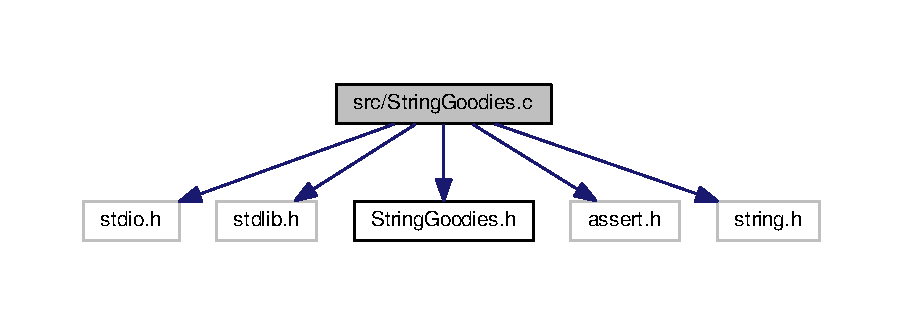
\includegraphics[width=350pt]{StringGoodies_8c__incl}
\end{center}
\end{figure}
\subsection*{Fonctions}
\begin{DoxyCompactItemize}
\item 
char $\ast$ \hyperlink{StringGoodies_8c_a205c8acb2ef70f038f32e5fe361cc8d9}{trimwhitespace} (char $\ast$str)
\begin{DoxyCompactList}\small\item\em fonction qui permet de supprimer les caracteres blancs en debut et en fin de chaine \end{DoxyCompactList}\item 
char $\ast$ \hyperlink{StringGoodies_8c_af59be06bfad0cf133ab6f4aca7b5b074}{str\+\_\+replace} (char $\ast$orig, char $\ast$rep, char $\ast$with)
\begin{DoxyCompactList}\small\item\em fonction qui permet de remplacer la chaine rep par with \end{DoxyCompactList}\item 
char $\ast$$\ast$ \hyperlink{StringGoodies_8c_ab39a39cfc3dafcdd137ec53ca81936d7}{str\+\_\+split} (char $\ast$a\+\_\+str, const char a\+\_\+delim)
\begin{DoxyCompactList}\small\item\em fonction qui permet de spliter une chaine par rapport a un caractere \end{DoxyCompactList}\item 
bool \hyperlink{StringGoodies_8c_a266480e602ae7b55989e10c1de0d53f2}{starts\+With} (const char $\ast$pre, const char $\ast$str)
\begin{DoxyCompactList}\small\item\em fonction qui permet de verifier si une chaine commence par une autre \end{DoxyCompactList}\end{DoxyCompactItemize}


\subsection{Description détaillée}
Fichier utilitaire créer pour faciliter le traitement des chaînes de caractères. 

\begin{DoxyAuthor}{Auteur}
Alexis Heil, Sabrina Bourouis 
\end{DoxyAuthor}
\begin{DoxyVersion}{Version}
0.\+1 
\end{DoxyVersion}
\begin{DoxyDate}{Date}
09 fevrier 2017
\end{DoxyDate}
Mini Shell de Sabrina Bourouis et Alexis Heil 

\subsection{Documentation des fonctions}
\index{String\+Goodies.\+c@{String\+Goodies.\+c}!starts\+With@{starts\+With}}
\index{starts\+With@{starts\+With}!String\+Goodies.\+c@{String\+Goodies.\+c}}
\subsubsection[{\texorpdfstring{starts\+With(const char $\ast$pre, const char $\ast$str)}{startsWith(const char *pre, const char *str)}}]{\setlength{\rightskip}{0pt plus 5cm}bool starts\+With (
\begin{DoxyParamCaption}
\item[{const char $\ast$}]{pre, }
\item[{const char $\ast$}]{str}
\end{DoxyParamCaption}
)}\hypertarget{StringGoodies_8c_a266480e602ae7b55989e10c1de0d53f2}{}\label{StringGoodies_8c_a266480e602ae7b55989e10c1de0d53f2}


fonction qui permet de verifier si une chaine commence par une autre 


\begin{DoxyParams}{Paramètres}
{\em char} & $\ast$ pre chaine par laquelle doit commencer str pour retourner 1 \\
\hline
{\em char} & str chaine dont il faut verifier qu\textquotesingle{}elle commence par pre \\
\hline
\end{DoxyParams}
\begin{DoxyReturn}{Renvoie}
int 1 si str commence par rep, 0 sinon 
\end{DoxyReturn}
\index{String\+Goodies.\+c@{String\+Goodies.\+c}!str\+\_\+replace@{str\+\_\+replace}}
\index{str\+\_\+replace@{str\+\_\+replace}!String\+Goodies.\+c@{String\+Goodies.\+c}}
\subsubsection[{\texorpdfstring{str\+\_\+replace(char $\ast$orig, char $\ast$rep, char $\ast$with)}{str_replace(char *orig, char *rep, char *with)}}]{\setlength{\rightskip}{0pt plus 5cm}char$\ast$ str\+\_\+replace (
\begin{DoxyParamCaption}
\item[{char $\ast$}]{orig, }
\item[{char $\ast$}]{rep, }
\item[{char $\ast$}]{with}
\end{DoxyParamCaption}
)}\hypertarget{StringGoodies_8c_af59be06bfad0cf133ab6f4aca7b5b074}{}\label{StringGoodies_8c_af59be06bfad0cf133ab6f4aca7b5b074}


fonction qui permet de remplacer la chaine rep par with 


\begin{DoxyParams}{Paramètres}
{\em char} & $\ast$ orig chaine dans laquelle il faut remplacer rep par with \\
\hline
{\em char} & $\ast$ rep chaine a remplacer \\
\hline
{\em char} & $\ast$ with chaine par laquelle on va remplacer rep \\
\hline
\end{DoxyParams}
\begin{DoxyReturn}{Renvoie}
char$\ast$ la chaine modifiee 
\end{DoxyReturn}
\index{String\+Goodies.\+c@{String\+Goodies.\+c}!str\+\_\+split@{str\+\_\+split}}
\index{str\+\_\+split@{str\+\_\+split}!String\+Goodies.\+c@{String\+Goodies.\+c}}
\subsubsection[{\texorpdfstring{str\+\_\+split(char $\ast$a\+\_\+str, const char a\+\_\+delim)}{str_split(char *a_str, const char a_delim)}}]{\setlength{\rightskip}{0pt plus 5cm}char$\ast$$\ast$ str\+\_\+split (
\begin{DoxyParamCaption}
\item[{char $\ast$}]{a\+\_\+str, }
\item[{const char}]{a\+\_\+delim}
\end{DoxyParamCaption}
)}\hypertarget{StringGoodies_8c_ab39a39cfc3dafcdd137ec53ca81936d7}{}\label{StringGoodies_8c_ab39a39cfc3dafcdd137ec53ca81936d7}


fonction qui permet de spliter une chaine par rapport a un caractere 


\begin{DoxyParams}{Paramètres}
{\em char} & $\ast$ a\+\_\+str chaine a spliter \\
\hline
{\em char} & a\+\_\+delim caractere par rapport auquel il faut spliter \\
\hline
\end{DoxyParams}
\begin{DoxyReturn}{Renvoie}
char$\ast$$\ast$ un tableau de la chaine splitee 
\end{DoxyReturn}
\index{String\+Goodies.\+c@{String\+Goodies.\+c}!trimwhitespace@{trimwhitespace}}
\index{trimwhitespace@{trimwhitespace}!String\+Goodies.\+c@{String\+Goodies.\+c}}
\subsubsection[{\texorpdfstring{trimwhitespace(char $\ast$str)}{trimwhitespace(char *str)}}]{\setlength{\rightskip}{0pt plus 5cm}char$\ast$ trimwhitespace (
\begin{DoxyParamCaption}
\item[{char $\ast$}]{str}
\end{DoxyParamCaption}
)}\hypertarget{StringGoodies_8c_a205c8acb2ef70f038f32e5fe361cc8d9}{}\label{StringGoodies_8c_a205c8acb2ef70f038f32e5fe361cc8d9}


fonction qui permet de supprimer les caracteres blancs en debut et en fin de chaine 


\begin{DoxyParams}{Paramètres}
{\em char} & $\ast$ str chaine dont il faut supprimer les espaces \\
\hline
\end{DoxyParams}
\begin{DoxyReturn}{Renvoie}
char$\ast$ la chaine modifiee 
\end{DoxyReturn}

%--- End generated contents ---

% Index
\backmatter
\newpage
\phantomsection
\clearemptydoublepage
\addcontentsline{toc}{chapter}{Index}
\printindex

\end{document}
